\documentstyle[color,subfigure,graphicx,epsf,here,cite,otf,comment,nccmath,mediabb,fancyhdr,12pt]{jarticle}

\graphicspath{{./pic/}}
%%%\documentstyle{jarticle}
\setlength{\textwidth}{16.2cm}%A4
\setlength{\textheight}{23cm}%A4
\setlength{\topmargin}{-1.5cm}
\setlength{\oddsidemargin}{0cm}
\setlength{\evensidemargin}{0cm}
\setlength{\parskip}{1pt}
%\pagestyle{myheadings}
\pagestyle{fancy}
\lhead[名前]{名前}
\rhead[\today]{\today}
\title{新人ゼミ課題}
\author{名前}
\date{\today}

\begin{document}
	
	\maketitle
	\vspace*{20pt}

	\begin{center}
		{\LARGE \bf 基本課題}
	\end{center}
    %\setcounter{section}{0}
    \addtocounter{section}{-1}
	\section{python+OpenCVの環境構築}
	%本文
	あ
	\section{Matを使った四則演算}
	\begin{figure}[h]
		%\begin{minipage}{\hsize}
		\begin{center}
			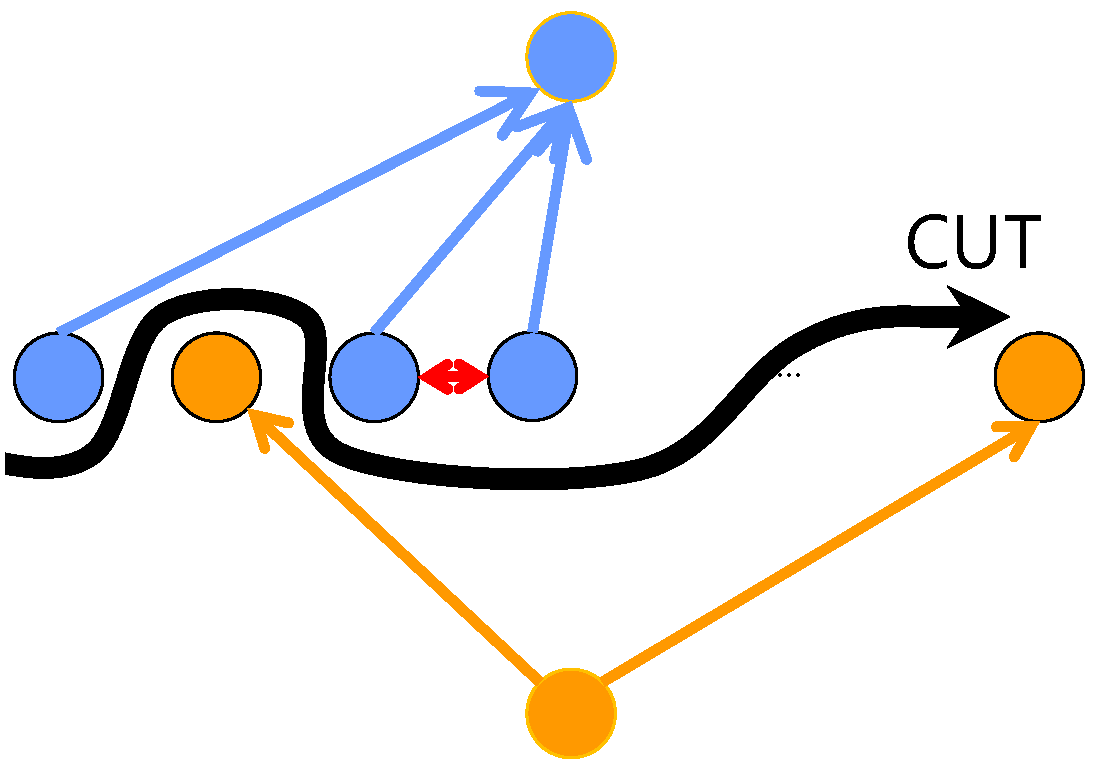
\includegraphics[width=0.4\hsize]{a.pdf}
			\caption{あ}
			\label{Kinect_Coordinate_system}
		\end{center}
		%\end{minipage}
	\end{figure}
	
	\newpage
	\begin{center}
		{\LARGE \bf 応用課題}
	\end{center}
	
	%本文
	い
	
	
	
	
\end{document}
